\documentclass[11pt,a4paper,oneside]{book}
\usepackage{a4wide}                     % Iets meer tekst op een bladzijde
\usepackage[dutch]{babel}               % Voor nederlandstalige hyphenatie (woordsplitsing)
\usepackage{amsmath}                    % Uitgebreide wiskundige mogelijkheden
\usepackage{amssymb}                    % Voor speciale symbolen zoals de verzameling Z, R...
\usepackage{makeidx}                    % Om een index te maken
\usepackage{url}                        % Om url's te verwerken
\usepackage{graphicx}                   % Om figuren te kunnen verwerken
\usepackage[small,bf,hang]{caption}     % Om de captions wat te verbeteren
\usepackage{xspace}                     % Magische spaties na een commando
\usepackage[latin1]{inputenc}           % Om niet ascii karakters rechtstreeks te kunnen typen
\usepackage{float}                      % Om nieuwe float environments aan te maken. Ook optie H!
\usepackage{flafter}                    % Opdat floats niet zouden voorsteken
\usepackage{listings}                   % Voor het weergeven van letterlijke text en codelistings
\usepackage[round]{natbib}              % Voor auteur-jaar citaties.
\usepackage[nottoc]{tocbibind}		% Bibliografie en inhoudsopgave in ToC; zie tocbibind.dvi
\usepackage{eurosym}                    % om het euro symbool te krijgen
\usepackage{textcomp}                   % Voor onder andere graden celsius
\usepackage{fancyhdr}                   % Voor fancy headers en footers
\usepackage[Gray,squaren,thinqspace,thinspace]{SIunits} % Om elegant eenheden te zetten
\usepackage[version=3]{mhchem}          % Voor elegante scheikundige formules

\usepackage{pdfpages}					% Pdf includeren

\usepackage{nomencl}
\makenomenclature %update bij every run
\renewcommand{\nomname}{Lijst van afkortingen}

% Volgend package is niet echt nodig. Het laat echter toe om gemakkelijk elektronisch
% te navigeren in je pdf-document. Deze package moet altijd als laatste ingeladen worden.
\usepackage[a4paper,plainpages=false]{hyperref}    % Om hyperlinks te hebben in het pdfdocument.


%%%%%%%%%%%%%%%%%%%%%%%%%%%%%%
% Algemene instellingen van het document.
%%%%%%%%%%%%%%%%%%%%%%%%%%%%%%

% De splitsingsuitzonderingen
\hyphenation{back-slash split-sings-uit-zon-de-ring}

%\bibpunct{(}{)}{;}{y}{,}{,}             % Auteur-jaar citaties -- zie natbib.dvi voor meer uitleg; niet echt nodig

% Het bibliografisch opmaak bestand.
% ZORG ERVOOR DAT bibliodutch.bst ZICH IN JE WERKDIRECTORY BEVINDT!!!
\bibliographystyle{bibliodutch}

\setlength{\parindent}{0cm}             % Inspringen van eerste lijn van paragrafen is niet gewenst.

\renewcommand{\baselinestretch}{1.2} 	% De interlinie afstand wat vergroten.

\graphicspath{{figuren/}}               % De plaars waar latex zijn figuren gaat halen.

\makeindex                              % Om een index te genereren.

\setcounter{MaxMatrixCols}{20}          % Max 20 kolommen in een matrix

% De headers die verschijnen bovenaan de bladzijden, herdefinieren:
\pagestyle{fancy}                       % Om aan te geven welke bladzijde stijl we gebruiken.
\fancyhf{}                              % Resetten van al de fancy settings.
\renewcommand{\headrulewidth}{0pt}      % Geen lijn onder de header. Zet dit op 0.4pt voor een mooie lijn.
\fancyhf[HL]{\nouppercase{\textit{\leftmark}}} % Links in de header zetten we de leftmark,
\fancyhead[HR]{\thepage}                % Rechts in de header het paginanummer.
% Activeer de volgende lijn en desactiveer de vorige om paginanummers onderaan gecentreerd te krijgen.
%\fancyhf[FC]{\thepage}                  % Paginanummers onderaan gecentreerd.

% PDF specifieke opties, niet strict noodzakelijk voor een thesis.
% Is hetgeen verschijnt wanneer je in acroread de documentproperties bekijkt.
\hypersetup{
    pdfauthor = {Andreas De Lille},
    pdftitle = {Automatische testbed monitoring voor toekomstig internet onderzoek met jFed},
    pdfsubject = {Scriptie van de masterproef Automatische testbedmonitoring voor toekomstig internet onderzoek met jFed},
    pdfkeywords = {testbed, jFed, monitoring, webservice, eindwerk, scriptie}
}


% Het volgende commando zou ervoor moeten zorgen dat er een witte ruimte wordt gelaten tussen
% elke paragraaf. Het zorgt ervoor dat er echter teveel witte ruimte komt boven en onder de
% verschillende titels, gemaakt met \section, subsection...
%%\setlength{\parskip}{0ex plus 0.3ex minus 0.3ex}

% Vandaar dat we expliciet aangeven wanneer we wensen dat een nieuwe paragraaf begint:
% \par zorgt ervoor dat er een nieuwe paragraaf begint en
% \vspace zorgt voor vertikale ruimte.
\newcommand{\npar}{\par \vspace{2.3ex plus 0.3ex minus 0.3ex}}

%%%%%%%%%%%%%%%%%%%%%%%%%%%%%%
% Nieuwe commando's
%%%%%%%%%%%%%%%%%%%%%%%%%%%%%%

% De differentiaal operator
\newcommand{\diff}{\ensuremath{\mathrm{d}}} 

% Super en subscript
\newcommand{\supsc}[1]{\ensuremath{^{\text{#1}}}}   % Superscript in tekst
\newcommand{\subsc}[1]{\ensuremath{_{\text{#1}}}}   % Subscript in tekst

% Chemische formule font:
\newcommand{\ch}[1]{\ensuremath{\mathrm{#1}}\xspace}	 
% Chemische pijl naar rechts:
\newcommand{\chpijlr}{\ensuremath{\hspace{1em}\longrightarrow\hspace{1em}}}
% Chemische pijl naar links:
\newcommand{\chpijll}{\ensuremath{\hspace{1em}\longleftarrow\hspace{1em}}}
% Chemische pijl naar links en rechts:
\newcommand{\chpijllr}{\ensuremath{\hspace{1em}\longleftrightarrow\hspace{1em}}}

\newcommand{\vt}[1]{\ensuremath{\boldsymbol{#1}}} % vector in juiste lettertype
\newcommand{\mx}[1]{\ensuremath{\mathsf{#1}}}	  % matrix in juiste lettertype

% Het latex logo in een eenvoudiger commando steken
\newcommand{\latex}{\LaTeX\xspace}

% Het BibTeX logo
\newcommand{\bibtex}{\textsc{Bib}\TeX\xspace}

% Niew commando om bestandnamen anders weer te geven
\newcommand{\bestand}[1]{\lstinline[basicstyle=\sl]{#1}\xspace}

% Niew commando om commando tekst weer te geven
\newcommand{\command}[1]{\lstinline[basicstyle=\tt]{#1}\xspace}
\newcommand{\commandx}[1]{\index{#1}\lstinline[basicstyle=\tt]{#1}\xspace}

%\lstset{morecomment={\%}}
% Commando om latex commando`s weer te geven (x: voor indexing)
%\newcommand{\lcommand}[1]{\lstinline[basicstyle={\tt},{language=[LaTeX]TeX}]{#1}\xspace}
\newcommand{\lcommand}[1]{\lstinline[basicstyle={\tt}]{#1}\xspace}
\newcommand{\lcommandx}[1]{\index{#1}\lstinline[basicstyle=\tt]{#1}\xspace}


% Niew commando om vreemde taal weer te geven (hint: dit commando kan gebruikt
%   worden om latijnse namen, die ook cursief moeten staan, weer te geven.
\newcommand{\engels}[1]{\textit{#1}\xspace}
\newcommand{\engelsx}[1]{\index{#1}\textit{#1}\xspace}

% Niew commando om iets te benadrukken en tegelijkertijd in de index te steken.
\newcommand{\begrip}[1]{\index{#1}\textbf{#1}\xspace}

% Nieuw commando om figuren in te voegen. Gebruik:
% \mijnfiguur[H]{width=5cm}{bestandsnaam}{Het bijschrift bij deze figuur}
\newcommand{\mijnfiguur}[4][ht]{            % Het eerste argument is standaar `ht'.
    \begin{figure}[#1]                      % Beginnen van de figure omgeving
        \begin{center}                      % Beginnen van de center omgeving
            \includegraphics[#2]{#3}        % Het eigenlijk invoegen van de figuur (2: opties, 3: bestandsnaam)
            \caption{#4\label{#3}}          % Het bijschrift (argument 4) en het label (argument 3)
        \end{center}
    \end{figure}
    }

% Nieuw commando om figuren in te voegen. Gebruik:
% \mijnfiguur[H]{bestand-tabular}{Het bijschrift bij deze tabel}    
\newcommand{\mijntabel}[3][ht]{             % Het eerste argument is standaar `ht'.
    \begin{table}[#1]                       % Beginnen van de table omgeving
        \begin{center}                      % Beginnen van de center omgeving
            \caption{#3\label{#2}}          % Het bijschrift (argument 3) en het label (argument 2)
            \input{#2}                      % Invoer van de tabel
        \end{center}
    \end{table}
}

%quoten
\newcommand{\quotes}[1]{\lq #1\rq\xspace}

%%%%%%%%%%%%%%%%%%%%%%%%%%%%%%
% Nieuwe wiskunde operatoren
%%%%%%%%%%%%%%%%%%%%%%%%%%%%%%

\DeclareMathOperator{\integ}{Integraal}

%%%%%%%%%%%%%%%%%%%%%%%%%%%%%%
% Nieuwe omgevingen
%%%%%%%%%%%%%%%%%%%%%%%%%%%%%%

% Een soort theorem omgeving
\newtheorem{levensles}{Levensles}[chapter]

% Om minder belangrijke delen iets kleiner te zetten.
\newenvironment{MinderBelangrijk}{\small}{}

% Een nieuwe omgeving om letterlijke latex tekst weer te geven.
\lstnewenvironment{llt} 
    {
    \vspace{1.2ex plus 0.5ex minus 0.5ex}   % Beetje ruimte voor de letterlijke tekst
    \lstset{                                % Enkele opties:
        basicstyle={\small\tt},             % Iets kleiner
        %language=[LaTeX]{TeX},              % Syntax highlighting
        stepnumber=0,                       % De lijnen worden niet genummerd
        breaklines=true,                    % Als een lijn te lang is, wordt hij afgebroken
        basewidth={0.5em},                  % Breedte van een letter
        xleftmargin=1em}                    % Inspringing van de linker marge
    }
    {\vspace{0.9ex plus 0.5ex minus 0.5ex}  % Beetje ruimte na de letterlijke tekst
    }

% Een nieuwe omgeving om algemene letterlijke tekst weer te geven.
\lstnewenvironment{lt} 
    {
    \vspace{1.2ex plus 0.5ex minus 0.5ex}   % Beetje ruimte voor de letterlijke tekst
    \lstset{                                % Enkele opties:
        basicstyle={\small\tt},             % Iets kleiner en typmachine lettertype
        stepnumber=0,                       % De lijnen worden niet genummerd
        breaklines=true,                    % Als een lijn te lang is, wordt hij afgebroken
        basewidth={0.5em},                  % Breedte van een letter
        xleftmargin=1em}                    % Inspringing van de linker marge
    }
    {\vspace{0.9ex plus 0.5ex minus 0.5ex}  % Beetje ruimte na de letterlijke tekst
    }



%%%%%%%%%%%%%%%%%%%%%%%%%%%%%%
% Einde van de preamble.
% Begin van de body:
%%%%%%%%%%%%%%%%%%%%%%%%%%%%%%

\begin{document}

\frontmatter

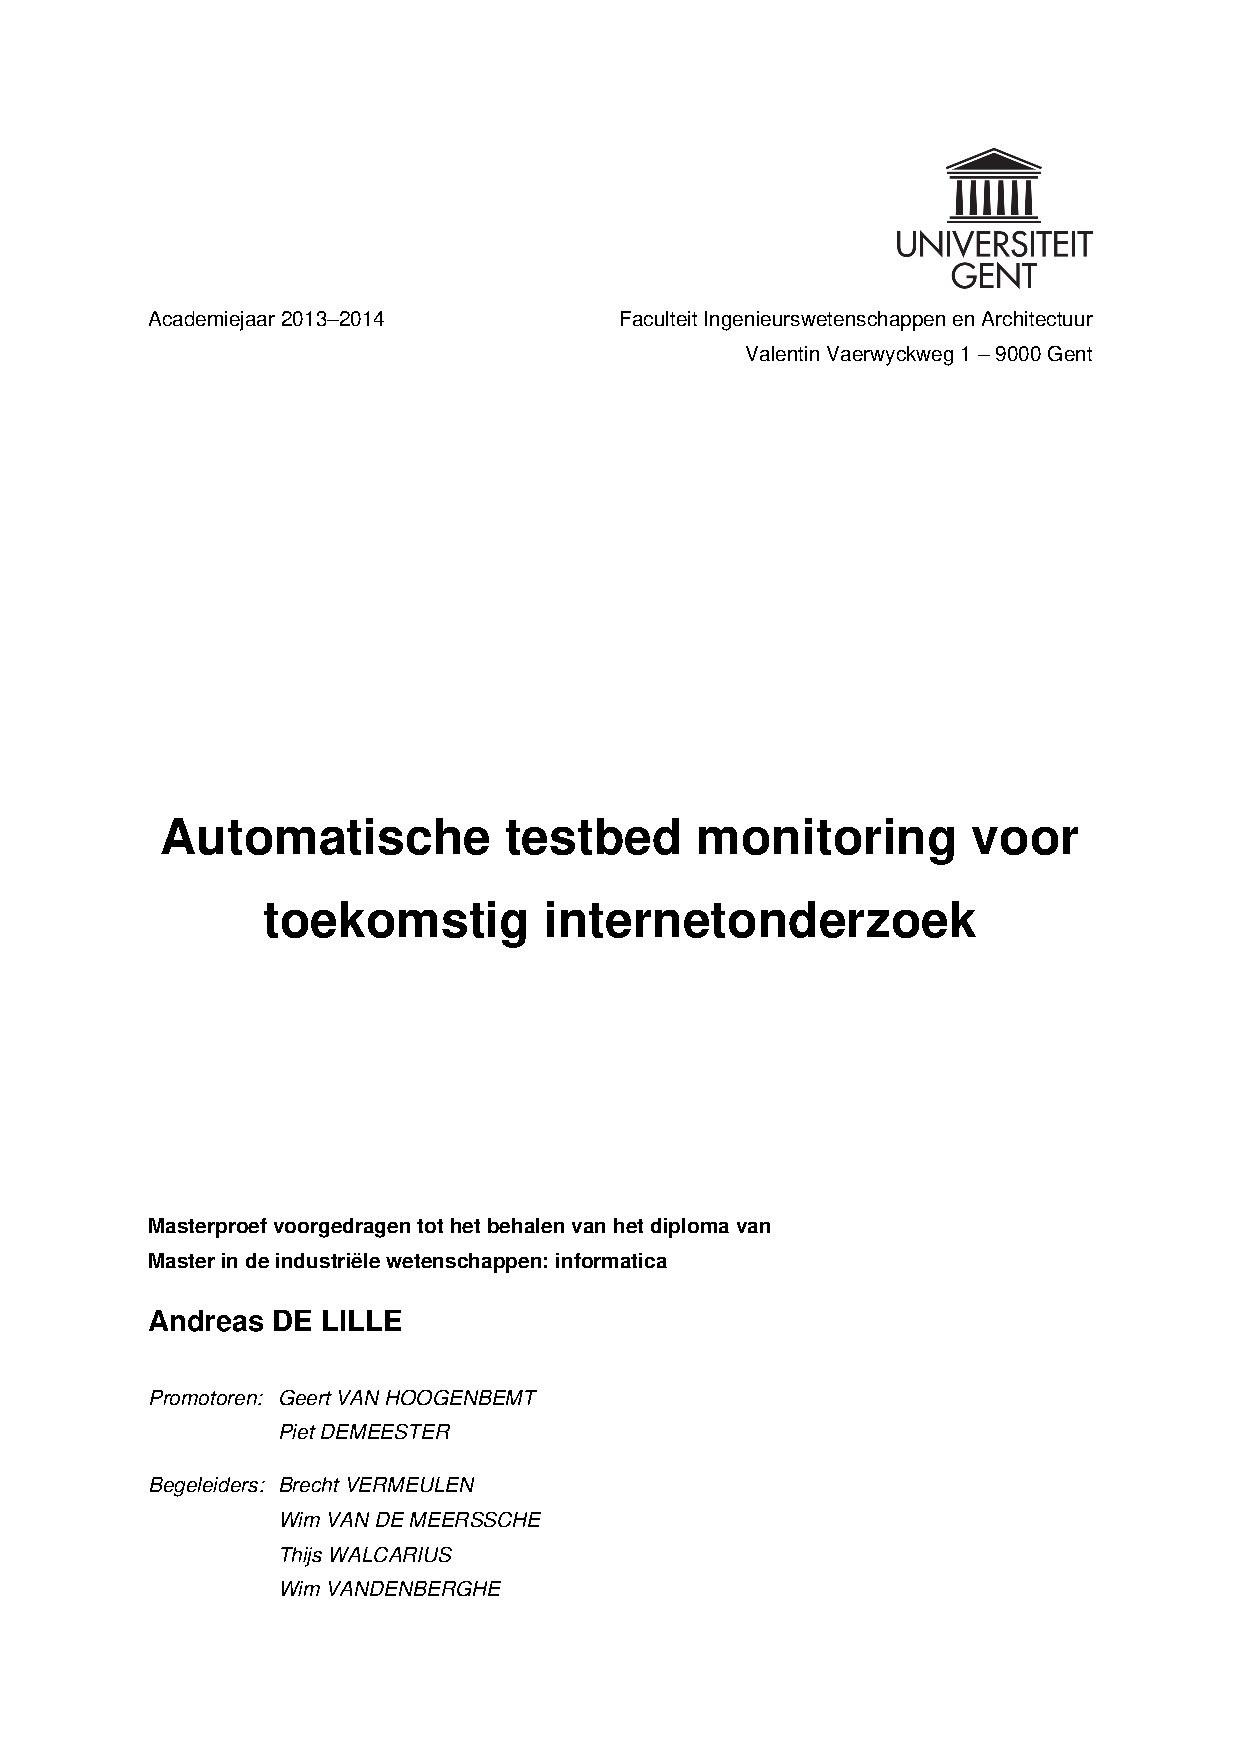
\includepdf[pages={1}]{titelblad.pdf}       %titelblad

%
% Typisch copyright voor een thesis.
% Te plaatsen juist na het titelblad.

\rule[-0.4\baselineskip]{0cm}{10\baselineskip}   
\par \vspace{2.3ex plus 0.3ex minus 0.3ex}
De auteur en promotor geven de toelating deze scriptie voor consultatie beschikbaar te stellen en delen ervan te kopi�ren voor persoonlijk gebruik. Elk ander gebruik valt onder de beperkingen van het auteursrecht, in het bijzonder met betrekking tot de verplichting uitdrukkelijk de bron te vermelden bij het aanhalen van resultaten uit deze scriptie.
\par \vspace{2.3ex plus 0.3ex minus 0.3ex}
The author and promoter give the permission to use this thesis for consultation and to copy parts of it for personal use. Every other use is subject to the copyright laws, more specifically the source must be extensively specified when using from this thesis.
\par \vspace{2.3ex plus 0.3ex minus 0.3ex}
Gent, Juni 2004 % Vul de juiste datum in!!!
\par \vspace{2.3ex plus 0.3ex minus 0.3ex}

De promotor \hfill De begeleider \hfill De auteur
\npar
\vspace{2cm}
\npar
% Pas de volgende lijn aan!!!
Prof. dr. ir. A. Armagneau \hfill Zijnen assistent \hfill Gaspard Lequeux

\thispagestyle{empty} 

                   	% Voor een echte thesis.
%\newpage
%\mbox{}\vspace{-1cm}
%\thispagestyle{plain}

%\textbf{\Huge{Woord vooraf}}

\chapter*{Woord vooraf}

%\vspace{2cm}

\begin{slshape}

%\small
Deze cursus werd in November 2003 voor het eerst uitgegeven in het kader van een Zeus (Studenten Werkgroep Informatica) initiatief om thesistudenten te helpen hun thesis in een aantrekkelijke vorm te gieten. De tekst is opgevat als een soort minithesis zodat studenten gemakkelijk alles kunnen overnemen. Om die reden zijn de bronbestanden beschikbaar gemaakt op het internet.\footnote{\url{http://zeus.ugent.be/~gaspard/latex}} 
\npar
Hoewel sommige deeltjes van deze cursus expliciet gericht zijn op het maken van een thesis, kan de tekst gebruikt worden als algemene inleiding op \latex. In 2004 zag ook Prof. Ottoy dit in. Vandaar dat deze cursus nu deel uitmaakt van de lessen informatica in de tweede bachelor bio-ir van de Universiteit Gent. Bij die gelegenheid heeft hij de cursus volledig nagekeken op taalfouten, waarvoor dank.
\npar
In 2006 heeft Prof. Dawyndt de cursus ook grondig herlezen en nagekeken, waarvoor dank. Sindsdien wordt deze cursus gebruikt in de lessen Computergebruik gegeven in de eerste bachelor Informatica van de Universiteit Gent.
\npar
Voor het schrijven van deze handleiding \latex, werd gebruik gemaakt van twee werken: \textsf{A guide to \latex} van \citet{kopka99} en \textsf{Handleiding \latex} van Piet van Oostrum (1996). Uit dit laatste werden zelfs hele paragrafen overgenomen. Daarnaast werd natuurlijk rijkelijk geput uit de documentatie die meegeleverd wordt met \latex zelf.
\npar
Minder belangrijke delen worden in een kleiner lettertype weergegeven. Verder zijn er verschillende voetnoten die verwijzen naar \latex documentatie op een Debian GNU/Linux systeem. Niemand gebruikt dat natuurlijk. Maar de bedoeling ervan is dat de lezer weet dat de documentatie bestaat, welke bestandsnaam die heeft en waar ongeveer die te vinden is in de \latex directorystructuur. Het is dan niet zo moeilijk meer om in je favoriete besturingssysteem te zoeken naar de desbetreffende bestandsnaam. 
\npar
In een standaard MikTeX installatie (d\'e \latex distributie voor Windows), zijn de helpfiles van de verschillende \latex packages te vinden in \bestand{C:\\texmf\\doc\\latex}. In \bestand{C:\\texmf\\doc\\guides} zijn enkele algemene handleidingen te vinden over \latex.
\npar
Het woord vooraf dient ook om mensen te bedanken: 

\begin{itemize}

\item De mensen van Zeus, voor de stimulerende Vrije--\engels{Open Source} sfeer en het organiseren van lessen hier rond. 

\item Schamper, het studentenblad van de Universiteit Gent, voor het leveren van de promotor van dit werk.

\item Rudy Gevaert, die in het academiejaar 2001-2002 als eerste een \latex les gaf.

\item Geert Vernaeve, voor het eerste contact met \latex en het C-voorbeeld op bladzijde \pageref{cvoorbeeld}.

\item Mensen die fouten rapporteerden en/of verbeteringen suggereerden: David De Wolf, Annelies Huyck, Yves Nevelsteen, Stijn Gors, Geert Vernaeve, Michiel Meire, Hendrik Maryns, Olivier Verhoogen, Jean-Pierre Ottoy, Hugo Coolens, Lieven Clement, Andy Peene, Reinout Debergh, Frederik De Schrijver, David van der Ha, Brecht Donckels, Dominique Lebbe, Christopher De Dobbelaere, Paul Vogels, Heidi Vanparys, Stijn Depuydt, Veerle Gevaert, Joke Van Hevele, Katrien De Dauw, Francis Santens, Nicolas Vanden Bossche en Peter Dawyndt.

\item De (thesis)studenten van het Boerenkot,
%\footnote{Ook nog wel Faculteit Landbouwkundige en Toegepaste Biologische Wetenschappen genoemd, maar niemand gebruikt die lange naam ;-)}
die in 2003 gevraagd hebben naar deze handleiding.

\end{itemize}

\latex lijkt in het begin moeilijk: alles in tekstmode, geen knopjes, je moet speciale commando's kennen om iets te bereiken~\ldots\ De eerste dagen zul je inderdaad enkele problemen ondervinden. Zoeken, doorbijten en hulp vragen aan meer ervaren gebruikers zullen ervoor zorgen dat je na enkele weken zelfs je wiskundige redeneringen rechtstreeks in \latex uitvoert. 
\npar
Deze handleiding is waarschijnlijk niet fautloos. Het rapporteren van meer dan ��n fout, zorgt voor je naam in de volgende editie van dit woord vooraf. Ook inhoudelijke opmerkingen zijn steeds welkom.

\vspace{4ex}

\hfill Gaspard Lequeux

\hfill Gent 9 Augustus 2006

%\normalsize
\end{slshape}

                      	% Algemene versie

% Voor een echte thesis, komt hier de samenvatting...
\newpage
\chapter*{Abstract}
\npar
Door de huidige verschuiving naar cloud-gebaseerde technologi\"en zal het belang 
van netwerkprotocollen en beschikbaarheid van netwerken alleen maar toenemen.
Om deze verschuiving vlot te laten verlopen is er meer en meer onderzoek nodig naar netwerktechnologi\"en.
Voor dit onderzoek wordt er dan ook veelvuldig gebruik gemaakt van testbeds.
Testbeds worden aangestuurd via jFed en worden gebruikt om netwerken te simuleren.
De situatie heeft enkele nadelen. Het is voor een onderzoeker soms erg moeilijk om te bepalen of een bepaald gedrag in hun experiment te wijten is aan de eigen ontwikkelingen, of aan het testbed zelf.
\npar
Deze masterproef zal trachten dit probleem te verhelpen door de testbed monitoring te automatiseren. Via een webservice zal deze informatie dan aangeboden worden. Deze webservice zal weergeven hoe betrouwbaar een testbed is. Hiervoor komen verschillende ontwikkelingstools aan bod. Uiteindelijk zal deze service ervoor zorgen dat een onderzoeker via zijn primaire gebruikersinterface op de hoogte gebracht wordt van eventuele problemen.                            % ...in het Nederlands en...
\newpage
\chapter*{Abstract}
\npar
Due to the new cloud-based technologies, network protocols and network reachability are now more important than ever. To make this change quick and clean, we need more and more network research. FIRE (Future Internet Research and Experimentation) is an European project created to improve the network and internet experimentation. FIRE is the opportunity to jointly develop potentially disruptive innovations for the future of the internet. It is about collaborative research and sharing test facilities. Researchers working for FIRE will now work closer together, sharing ideas. FIRE is also used to share test facilities from all over the world, so researchers have access to many different test facilities.\\

To make handling of these different testbeds easier, jFed was created. jFed is a java tool with the purpose of controlling testbeds. Unfortunately, the current situation has a major downside in that it is very hard for researchers to determine if a certain behavior is caused by the testconfiguration or by the test facility. 
\npar
This thesis will try to solve the aforementioned problem by creating an automated the testbed monitoring system. A monitoringAPI will then share this information. Doing so, will provide future tools easy access to this information.                            % ...in het Engels.
%voorwoord?
%dankwoord?/back	

%afkortingen
\printnomenclature

%figuren
\listoffigures
%tabellen
\listoftables

% De lijnen van de inhoudsopgave iets dichter op elkaar, niet echt nodig voor de thesis, maar 
% voor dit werk kregen we anders een laatste bladzijde met 3 items op.
\renewcommand{\baselinestretch}{1.08} 	% De interlinie afstand wat vergroten.
\small\normalsize                       % Nodig om de baselinestretch goed te krijgen.
\tableofcontents
\renewcommand{\baselinestretch}{1.2} 	% De interlinie afstand wat vergroten.
\small\normalsize                       % Nodig om de baselinestretch goed te krijgen.

\mainmatter

% De verschillende hoofdstukken:
\newpage
\chapter{Inleiding}
\section{Bestaande situatie}
\npar
iMinds is een onafhankelijk onderzoekscentrum dat opgericht werd door de Vlaamse overheid.
Het is voornamelijk bezig met onderzoek omtrent ICT-innovatie. Bij dit onderzoek wordt veelvuldig gebruik gemaakt van testbeds. Een testbed is een verzameling van nodes waarmee netwerkopstellingen kunnen gesimuleerd worden. 
\npar
Een goed voorbeeld van een testbed is de Virtual Wall. De Virtual Wall is ontworpen voor het experimenteren met nieuwe netwerkoplossingen voor de volgende generatie van het Internet. De kracht van deze infrastructuur is dat ze de mogelijkheid biedt om op een eenvoudige wijze specifieke netwerkopstellingen op te zetten volgens de noden van het onderzoek. 
\npar
Een voorbeeld waarvoor dit testbed wordt gebruikt is dat men een server en een aantal cli\"ents definieert. Deze worden verbonden met een aantal tussenliggende routers. Vervolgens wordt een videostream opgestart. Op deze videostream kan men storing introduceren door pakketten te droppen. Deze storing zal ervoor zorgen dat het beeld aan de client-side hapert. Er kunnen technieken ingebouwd worden aan client-side om deze storing op te vangen. Zo kan er overgeschakeld worden naar een lagere kwaliteit indien blijkt dat de beschikbare bandbreedte onvoldoende is. Testen van degelijke technieken verloopt dan ook aan de hand van testbeds.
\npar
Onderzoekers bij iMinds hebben niet alleen toegang tot hun Virtual Wall, maar door samenwerkingsakkoorden met diverse onderzoekscentra hebben ze ook wereldwijd toegang tot andere en soms erg verschillende testbeds. Deze zijn elk apart ontwikkeld. Hierdoor maakt elk testbed gebruik van een eigen interface. Deze interface wordt aangeboden door middel van een federation API (application programming interface) \nomenclature{API}{application programming interface}. Een federation API is een interface die alle mogelijk functionaliteiten van een specifiek testbed aanbiedt. Hij staat in voor de communicatie tussen een programma en het testbed. Onderzoekers die met meerdere testbeds werken, moeten dan ook de werking van elk testbed apart bestuderen alvorens ermee aan de slag te kunnen. Ook rechtstreekse verbindingen leggen tussen verschillende testbeds wordt hierdoor moeilijker. 
\npar
Daarom werd in het Europese onderzoeksproject Fed4FIRE beslist om een aantal federation API's vast te leggen die gelijk moeten zijn op elk testbed. Dit maakt het mogelijk om tools te ontwikkelen die bruikbaar zijn op alle testbeds verenigd in dit project. Hiervoor werd de tool jFed ontwikkeld door iMinds. jFed biedt een wrapper aan rond de specifieke federation API's die in dat project worden toegepast. Daarenboven voorziet jFed in verschillende applicaties om enerzijds te kunnen testen of testbeds deze API's correct ondersteunen, en anderzijds om als onderzoeker op een eenvoudige wijze een experiment te kunnen opzetten. 
\npar
De kernmodule waar alle andere modules gebruik van maken is de "jFed library". De voornaamste functie van deze library is om de communicatie met de testbeds te vereenvoudigen. De hiervoor bruikbare testbeds implementeren enkele gestandaardiseerde API's, die de benodigde functionaliteiten aanbieden. De jFed library implementeert de client kant van deze API's (application programming interface), en voorziet Java interfaces voor de API-calls. De gebruiker zal hierdoor niet geconfronteerd worden met deze details. Zo zal de library o.a. de achterliggend SSL-connectie (secure sockets layer) \nomenclature{SSL}{secure sockets layer} en de bijhorende certificaten en private keys beheren. Verder zullen ook de nodige omzettingen gebeuren. Daarnaast bevat deze library vele hulpklassen en methoden om de API's aan te spreken.
\mijnfiguur{width=0.9\textwidth}{jFed}{Opbouw van jFed}
\npar
Een goed voorbeeld van een API die door jFed word ge\"implementeerd is de AM (Aggregate Manager) \nomenclature{AM}{Aggregate Manager} API, versie 2 en 3.  Een voorbeeld van een call, is de "CreateSliver" call in de AMv2 API.
De AMv2 API specificeert dat alle calls gedaan worden over een SSL verbinding met client-side certificaten. Verder specificeert de API de exacte argumenten die vereist zijn en het formaat van het resultaat. De jFed library biedt een Java methode "createSliver" in de klasse "AggregateManager2" aan. De argumenten worden opgegeven in een Java formaat. Zo zal bijvoorbeeld een datum-argument als een Java Date-object doorgegeven worden.  De jFed library zal de datum naar het RFC3339 formaat omzetten voor het naar de server verstuurd wordt. Ook het resultaat van de call wordt verwerkt door de jFed library terug omgezet.
\npar
Steunend op deze library zijn enkele tools zoals jFed probe en jFed compliance tester gebouwd. Deze hebben als doel het valideren of testbeds de federation API's correct ondersteunen. Tenslotte is er de jFed graphical user interface (GUI) \nomenclature{GUI}{graphical user interface} tool. Deze tool maakt het mogelijk om als eindgebruiker een experiment op een intu\"itieve manier op te zetten. De jFed GUI heeft momenteel echter een relatief complexe interface die gebruiksvriendelijker gemaakt kan worden. 

\section{Probleemstelling}
\npar
Er is echter nog ruimte voor verbetering in jFed. Zo worden er op geregelde tijdstippen verschillende testen automatisch uitgevoerd op testbeds. Deze testen geven o.a. weer of testbeds online zijn en of het aanmelden via een SSH-verbinding (secure shell)\nomenclature{SSH}{secure shell} gelukt is. Deze resultaten worden momenteel nog redelijk ad hoc bijgehouden. Men maakt geen gebruik van een databank, maar van bourne again shell (bash) \nomenclature{bash}{bourne again shell} scripts om de resultaten te archiveren. Resultaten op deze manier bijhouden, is uiteraard ineffici\"ent. Bovendien staat deze informatie momenteel enkel op een website vermeld. 
\npar
Een onderzoeker wordt dus niet via zijn primaire gebruikersinterface op de hoogte gebracht van eventuele storingen met de testbeds opgenomen in zijn experiment. Dit maakt het voor onderzoekers soms moeilijk om te identificeren of een bepaald gedrag in hun experiment te wijten is aan de eigen ontwikkelingen, of aan de testbeds zelf. Hierdoor kan veel tijd onnodig verloren gaan tijdens de uitvoering en de analyse van het experiment. Een betere oplossing zou zijn dat bij het selecteren van een testbed de betrouwbaarheid weergegeven wordt. Zo kan een betrouwbaar testbed gekozen worden, om dergelijke situaties zoveel mogelijk te vermijden.
\npar
Niet enkel de betrouwbaarheid is van belang, ook het \quotes{comfort} is van belang. Een testbed met een snellere verbinding geniet de voorkeur op een testbed met een trage verbinding. Naast de betrouwbaarheid en comfort moet ook gekeken worden naar de vereisten. Indien een betrouwbaar testbed niet beschikt over voldoende vrije resources, kan het niet gebruikt worden voor een experiment.
\npar
Door rekening houden met de betrouwbaarheid, het comfort en de vereisten kan jFed de onderzoeker melden dat een gekozen testbed niet betrouwbaar,niet beschikbaar of traag is. Hiervoor is een monitoringservice nodig. Programma's kunnen dan met api-calls de monitoringservice contacteren om te kijken welk testbed online is.
%achtergrond?
\newpage
\chapter{Analyse}
\section{Bestaande uitwerking}
\npar
De oplossing van dit probleem en tevens het onderwerp van mijn thesis is een webservice die de monitoring automatiseerd. Hierbij komen een aantal vragen naar boven. Welke informatie moet bijgehouden worden? 
Wat bepaald de betrouwbaarheid van een testbed? Hoe nauwkeurig moet deze informatie bijgehouden worden? 
\npar
De ontwikkeling van de huidige situatie is door de sneller ontwikkeling, minder gestructureerd verlopen.
Hierdoor bestaat de software uit een basis versie gevolgd door een aantal \quotes{quick and dirty} toevoegingen. Er moet opgemerkt worden dat de huidige situatie werkt, maar het kan beter. Het gemist van structuur in opbouw zal op lange termijn leiden tot code die zeer moeilijk aan te passen is.
\subsection{Databanken}
\npar
De huidige situatie voorziet niet in een centrale webservice.
Wat er wel bestaat is een verzameling websites die rechtstreeks verbinding maken met een of meerdere databanken. Er zijn 3 databanken voorzien:
\begin{enumerate}
\item flsmonitoring
\item flsmonitoring-international
\item scenarios
\end{enumerate}
\newpage
\subsubsection{flsmonitoring databank}
\npar
In de eerste en de tweede databank bestaan uit een tabel waarin de laatste resultaten van elke test bijgehouden worden. Het verschil tussen deze 2 databanken komt overeen met de toegewezen categorie waarin het testbed zich bevind. De eerste databank bevat de locale testbeds, de tweede bevat de internationale testbeds. Deze tabellen bevatten volgende kolommen:
\begin{itemize}
\item testbedid
\item testbedname
\item testbedurl
\item pinglatency
\item getversionstatus
\item aggregatetestbedstate
\item last-check
\end{itemize}
 De eerste 3 parameters zijn duidelijk. \quotes{Pinglatency} houdt de waarde van de pingtest bij.
De kolommen \quotes{getversionsStatus} en \quotes{aggregatetestbedstate} worden gebruikt om de uitkomst van de getVersion test bij te houden. Deze test bevat o.a. het versie nummer van de aggregate manager. Doordat er geen ssl authenticatie nodig is voor deze test, wordt hij vaak gebruikt om de status van een server op te vragen. De kolom \quotes{last-check} bevat een timestamp om bij te houden waneer de lijn laatste werd aangepast.
\subsubsection{scenario databank}
\npar
De laatste databank bestaat uit 3 tabellen. Het doel ervan is het bijhouden van informatie over de scenariotesten. Scenariotesten of stitchingtesten zijn complexe testen die uit meerdere subtesten bestaan. Eenvoudig gezegd zal een stitching test de verbinding tussen verschillende testbeds testen. Hiervoor worden op elk testbed meerdere resources aangevraagd. Deze zullen dan trachten naar elkaar te pingen. Indien een testbed offline is wordt de volledige test afgebroken. Hieronder staan de opeenvolgende stappen die een stitching of scenariotest doorloopt.
\begin{enumerate}
\item setUp
\item getUserCredential
\item generateRspec
\item createSlice
\item initStitching
\item callSCS
\item callCreateSlivers
\item waitForAllReady
\item loginAndPing
\item callDeletes
\end{enumerate}
De inhoud van elke subtest wordt hier buiten beschouwing gelaten.
Wat wel opgemerkt kan worden is dat we de tests kunnen opdelen in 3 groepen. Zo zijn testen 1-6 voorbereidende testen. Ze dienen om de configuratie voor testen 7-9 klaar te zetten. Test 10 is de cleanup die de opgebouwde configuratie van stappen 1-6 terug ongedaan maakt.
Elke subtest heeft een resultaat. Een stitching test zou dus minstens 10 resultaten hebben. In de huidige versie zijn er slechts 3 statussen gedefini\"eerd. De stitching test is volledig gelukt, dit komt overeen met 10 geslaagde subtests. De status is gedeeltelijk gelukt, dit komt overeen met de voorbereiding die wel gelukt is, maar de stappen 7-9 zijn niet of slechts gedeeltelijk gelukt. De laatste status geeft aan dat alle subtests mislukt zijn.
\npar
De database is opgebouwd uit 3 tabellen.
\begin{itemize}
\item test-results
\item test-context
\item testbeds
\end{itemize}
De eerste resultaat houdt informatie bij over de testresultaten. De tweede tabel houdt de context van de test bij. De laatste tabel houdt de testbeds bij. De concrete invulling van de tabellen zou ons te ver leiden.
\clearpage
\section{Problemen in de huidige uitwerking}
\npar
Een eerste situatie die beter kan is het bijhouden van de laatste resultaten.
Deze resultaten zitten in een databank, die voor elke testbed een lijn bevat. Nieuwe waarde overschrijven die lijn. Meteen kan opgemerkt worden dat het niet mogelijk is om statistieken over een lange termijn weer te geven.Het aanpassen van de monitoring waarden gebeurd door shell scripts. Deze worden periodiek uitgevoerd en lezen een configuratiefile in. Indien het testbed waarop de test uitgevoerd moet worden al in de databank zit is het id vermeld in de configuratiefile. Indien er geen id staat zal het script zelf een nieuwe lijn aanmaken en vervolgens de id wegschrijven naar de file. Eenmaal uitgevoerd, geeft de test een resultaat terug in de vorm van een xmlfile die door ge\"instaleerde commando\rq s geparset wordt. Vervolgens wordt de data weggeschreven naar de databank.
\npar


\section{aanpassingen}
opdeling van internation <-> gwn weg
opdeling flsmoni <-> scenarios weg

\section{besluit}
%use cases?
\newpage
\chapter{Ontwerp service}

In dit hoofdstuk wordt de interface van de webservice besproken. Daarna worden er enkele voorbeelden van calls uitgewerkt.

\section{Api Calls}
De calls kunnen opgedeeld worden in 2 grote groepen.
\begin{itemize}
\item Results: Het opvragen van resultaten van een test.
\item Configuration: Het opvragen, aanpassen en aanmaken van testen en de bijhorende configuratie.
\end{itemize}

\section{Calls - Results}
Voor het opvragen van resultaten wordt gebruik gemaakt van een generische functie.

\subsection{Functies}
Er zijn een aantal functies voorzien voor het opvragen van de resultaten.
\begin{itemize}
\item last: Deze functie geeft het laatste/ de laatste resultaat/resultaten terug (per test,testbed).
\item list: Deze functie geeft een lijst resultaten die voldoen aan de opgegeven parameters. 
Zo kan deze lijst bijvoorbeeld beperkt worden tot een resultaten die overeenkomen met een bepaalde status of vallen tussen bepaalde data.
%average weggelaten => enkel nuttig bij ping test dus mss niet nuttig
\item detail: Deze functie geeft een detailweergave terug van een test. Deze detail weergave kan bijvoorbeeld ook logfiles bevatten om debugging te vergemakkelijken.
\end{itemize}

\subsection{Parameters}
Hier worden de parameters besproken. Deze parameters zullen het resultaat van de functies hierboven filteren.

\begin{itemize}
\item testbed: Deze parameter duidt een of meerdere testbeds aan.
\item testtype: Deze parameter duidt het type van de test aan.
\item status: Deze parameter duidt de status aan. Let op dit is per subtest.
\item count: Deze parameter geeft het aantal laatste resultaten aan dat teruggegeven moet worden. 
Ook wanneer er enkel een till opgegeven is, worden de laatste resultaten voor de opgegeven tijd teruggegeven.
Wanneer er enkel een from parameter opgegeven is, dan worden de eerste x resultaten startend vanaf de from terug gegeven.
\item from: Geeft aan vanaf welke timestamp er gezocht moet worden.
\item till: Geeft aan tot welke timestamp de resultaten gezocht moeten worden.
\item resultid: Geeft een of meerdere id\rq s van een testresultaat.
\item testname: De naam van de test. Voornamelijk nodig bij stitching tests omdat er daar meerdere testbeds in betrokken zijn.
\item instanceId: Filteren op de testinstantie, gelijkaardig aan de testname.
\item format: Deze parameter dient niet om de resultaten te filteren, maar om het formaat van het resultaat te bepalen. Standaard is dit json, later kan eventueel xml en/of csv toegevoegd worden.
\end{itemize}
Indien bij tests of bij testbeds de waarde all wordt gegeven, worden respectievelijk alle tests of alle testbeds teruggegeven. Ook opgeven van lijsten is mogelijk. Zo kunnen de resultaten van pingtest voor 2 verschillende testbeds opvraagd worden met een call, zie ook voorbeelden.
\clearpage

\subsection{Voorbeelden}
Hieronder worden een aantal voorbeelden van calls en bijhorende antwoorden geven.
Voorlopig zijn de voorbeelden beperkt tot het opvragen van data met behulp van HTTP GET requests.
\subsubsection{last?testbed=urn-testbed0\&testtype=ping\&count=2}
Deze call geeft voor testbed0 de laatste 2 ping resultaten terug.
\begin{verbatim}
{
    "177": {
        "testinstanceid": "1",
        "testtype": "ping",
        "testname": "ping voor testbed0",
        "log": "http:\/\/f4f-mon-dev.intec.ugent.be\/logs\/1\/1386",
        "timestamp": "2014-03-18 19:29:12.876569",
        "testbeds": [
            "urn-testbed0"
        ],
        "results": {
            "pingValue": "166"
        }
    },
    "155": {
        "testinstanceid": "1",
        "testtype": "ping",
        "testname": "ping voor testbed0",
        "log": "http:\/\/f4f-mon-dev.intec.ugent.be\/logs\/1\/1615",
        "timestamp": "2014-03-18 19:29:09.138309",
        "testbeds": [
            "urn-testbed0"
        ],
        "results": {
            "pingValue": "223"
        }
    }
}
\end{verbatim}

\clearpage
\subsubsection{last?testbed=ALL\&testtype=ping}
Deze call geeft voor elk testbed de laatste ping resultaten terug.
\begin{verbatim}
{   "177": {
        "testinstanceid": "1",
        "testtype": "ping",
        "testname": "ping voor testbed0",
        "log": "http:\/\/f4f-mon-dev.intec.ugent.be\/logs\/1\/1386",
        "timestamp": "2014-03-18 19:29:12.876569",
        "testbeds": [ "urn-testbed0" ],
        "results": { "pingValue": "166" }
    },"178": {
        "testinstanceid": "2",
        "testtype": "ping",
        "testname": "ping voor testbed1",
        "log": "http:\/\/f4f-mon-dev.intec.ugent.be\/logs\/2\/9739",
        "timestamp": "2014-03-18 19:29:12.889286",
        "testbeds": [ "urn-testbed1" ],
        "results": { "pingValue": "112" }
    },"187": {
        "testinstanceid": "11",
        "testtype": "ping",
        "testname": "ping voor testbed10",
        "log": "http:\/\/f4f-mon-dev.intec.ugent.be\/logs\/11\/4280",
        "timestamp": "2014-03-18 19:29:13.039074",
        "testbeds": [ "urn-testbed10" ],
        "results": { "pingValue": "106" }
    },"188": {
        "testinstanceid": "12",
        "testtype": "ping",
        "testname": "ping voor testbed11",
        "log": "http:\/\/f4f-mon-dev.intec.ugent.be\/logs\/12\/2792",
        "timestamp": "2014-03-18 19:29:13.055714",
        "testbeds": [ "urn-testbed11" ],
        "results": { "pingValue": "156" }
    }
    ...
}
\end{verbatim}

\subsubsection{last?testname=stitching2}
Deze functie geeft een detail resultaat terug van de stitchingtest met naam 'stitching2'.
\begin{verbatim}
Voorbeeld invoegen
\end{verbatim}

\subsubsection{list?from=2014-03-18T19:29:00\&till=2014-03-18T19:29:10\&testtype=ping\&testbed=urn-testbed1}
Deze call geeft een lijst van de pingtests tussen 2014-03-18 19:29:00 en 2014-03-18 19u29:10 op testbed1 terug.
\begin{verbatim}
{
    "156": {
        "testinstanceid": "2",
        "testtype": "ping",
        "testname": "ping voor testbed1",
        "log": "http:\/\/f4f-mon-dev.intec.ugent.be\/logs\/2\/2306",
        "timestamp": "2014-03-18 19:29:09.152291",
        "testbeds": [
            "urn-testbed1"
        ],
        "results": {
            "pingValue": "66"
        }
    },
    "134": {
        "testinstanceid": "2",
        "testtype": "ping",
        "testname": "ping voor testbed1",
        "log": "http:\/\/f4f-mon-dev.intec.ugent.be\/logs\/2\/1991",
        "timestamp": "2014-03-18 19:29:05.413795",
        "testbeds": [
            "urn-testbed1"
        ],
        "results": {
            "pingValue": "24"
        }
    },
    ...
}
\end{verbatim}

\section{Calls - configuration}
Deze calls hebben het doel om de configuratie van een test op te vragen.

\subsection{Functies}
Er zijn (uiteraard) ook een aantal functies voor het opvragen van de testconfiguratie.
\begin{itemize}
\item TestDefinition : Geeft de definitie van een testweer. Deze bevat informatie over de naam, het commando. Verder duidt deze definitie ook aan welke parameters er nodig zijn en welke waarden er terug gegeven worden. Deze waarden zijn echter niet ingevuld. Het is de bedoel om hier bijvoorbeeld te defini\"eren dat een pingtest bijvoorbeeld bestaat uit een ping commando en dat deze een time-out en een testbed moet meekrijgen. Samengevat kan gesteld worden dat dit de beschrijving van een type test is.
\item Testbed: Geeft een of meerdere testbeds aan waarop de testinstantie gedefini\"eerd moet worden.
\end{itemize}

Deze opsplitsing is noodzakelijk om flexibiliteit aan te bieden. 
Een ping test wordt op meerdere testbeds uitgevoerd. Door deze opbouw moet een ping test maar eenmalig gedefini\"eerd worden. Als we de uitwerking vergelijking met het model-view-controller pattern, geeft de definition de klasse, de instance kan gezien worden als een object van die klasse.

\subsection{Parameters}

\begin{itemize}
\item testtype: Deze parameter duidt aan welke testtype opgevraagd wordt.
\item testinstanceId: Deze parameter duidt aan welke instance opgevraagd wordt. Er is geen equivalente variant voor testdefinition, omdat het testtype daar de unieke id voorstelt.
\end{itemize}
Het is ook mogelijk om als waarde ALL of een lijst van id's op te geven.

\subsection{Voorbeelden}
Hieronder worden een aantal mogelijke calls weergegeven. Voorlopig zijn deze voorbeelden beperkt tot het opvragen van data via http get requests.

\clearpage
\subsubsection{testDefinition?testtype=stitch}
Deze call geeft de beschrijving van een stitching test terug.
\begin{verbatim}
{   "stitch": {
        "testcommand": "stitch",
        "parameters": {
            "topology": {
                "type": "string",
                "description": "ring | line"
            },"testbedId": {
                "type": "testbedId[]",
                "description": "multiple testbeds for ping test"
            }
        },"return": {
            "callDeletes": {
                "type": "string", "description": "status of subtest"
            },"loginAndPing": {
                "type": "string", "description": "status of subtest"
            },"waitForAllReady": {
                "type": "string", "description": "status of subtest"
            },"callCreateSlivers": {
                "type": "string", "description": "status of subtest"
            },"callSCS": {
                "type": "string", "description": "status of subtest"
            },"initStitching": {
                "type": "string", "description": "status of subtest"
            },"createSlice": {
                "type": "string", "description": "status of subtest"
            },"generateRspec": {
                "type": "string", "description": "status of subtest"
            },"getUserCredential": {
                "type": "string", "description": "status of subtest"
            },"setUp": {
                "type": "string", "description": "status of subtest"
}}}}
\end{verbatim}
\clearpage
\subsubsection{testInstance?testbed=urn-testbed1,urn-testbed2}
Hierbij worden alle testinstanties van testbed1 en testbed2 teruggegeven. Dit zijn dus de testen die effectief draaien op testbed1 en/of testbed2.
\begin{verbatim}
{    "2": {
        "testname": "ping voor testbed1",
        "testtype": "ping",
        "frequency": "60",
        "parameters": [
        	{"testbedId": "urn-testbed1"},
            {"timeout": "300"}
        ]
    },"3": {
        "testname": "ping voor testbed2",
        "testtype": "ping",
        "frequency": "60",
        "parameters": [
            {"testbedId": "urn-testbed2"},
            {"timeout": "300"}
        ]
    },"18": {
        "testname": "stiching0",
        "testtype": "stitch",
        "frequency": "3600",
        "parameters": [
            {"testbedId": "urn-testbed2"},
            {"testbedId": "urn-testbed1"},
            {"testbedId": "urn-testbed0"},
            {"topology": "ring"}
        ]
    },	
    ...    
}
\end{verbatim}
\clearpage
\subsubsection{testInstance?testtype=ping}
Deze call geeft alle geplande tests terug.
\begin{verbatim}
{
    "1": {
        "testname": "ping voor testbed0",
        "testtype": "ping",
        "frequency": "60",
        "parameters": [
            { "testbedId": "urn-testbed0" },
            { "timeout": "300" }
        ]
    },
    "2": {
        "testname": "ping voor testbed1",
        "testtype": "ping",
        "frequency": "60",
        "parameters": [
            { "testbedId": "urn-testbed1" },
            { "timeout": "300" }
        ]
    },
    "3": {
        "testname": "ping voor testbed2",
        "testtype": "ping",
        "frequency": "60",
        "parameters": [
            { "testbedId": "urn-testbed2" },
            { "timeout": "300" }
        ]
    },
    ...
}
\end{verbatim}
\newpage
\chapter{Ontwerp Databank}
In dit hoofdstuk wordt de interface van de databank besproken.

\section{Tabellen}
De database zal bestaan uit volgende tabellen.
\begin{itemize}
\item testbeds: Deze tabel zal informatie over de testbeds bijhouden.

\item testDefinitions: Deze tabel zal de testbeschrijving bijhouden.
\item parameterDefinitions: Deze tabel houdt de parameters bij die de test nodig heeft.
\item returnDefinitions: Deze tabel houdt de returnwaardes bij die een test genereert.

\item testInstances: Hier worden de instanties van de testdefinities bijgehouden. Deze tabel zorgt voor de link tussen de testdefinitie en de ingevulde parameters.
\item parameterInstances: Deze tabel houdt de ingevulde waarden van de parameters bij.

\item results: Deze tabel zorgt voor de link tussen de testinstantie en de subresults.
\item subResults: Deze tabel houdt de verschillende resultaten van een testbij.
\end{itemize}

Merk hier ook de opsplitsing testDefinition $<$=$>$ testInstance. TestDefinition is een definitie van een test, testinstantie is de test met de ingevulde waarden.

\section{Testbeds}
Deze tabel houdt de verschillende testbeds bij en bevat volgende kolommen :
\begin{itemize}
\item testbedId: Het id van het testbed. Dit veld moet uniek zijn voor elk testbed.
\item name: de naam van het testbed.
\end{itemize}

\section{TestDefinitions}
Deze tabel houdt de definities van de tests bij.
Hierbij wordt een test abstract omschreven als een commando met een aantal parameters en een of meerdere return waarden. De tabel bevat volgende kolommen:
\begin{itemize}
\item testtype : Dit is de naam van een testtype en moet tevens uniek zijn.
\item testcommand : Het commando (of script) dat uitgevoerd moet worden.
\end{itemize}
\section{ParameterDefinitions}
Deze tabel houdt bij welke parameters een test nodig heeft. Hierbij wordt de naam, het type en een beschrijving van een parameter opgeslagen. De tabel bevat volgende kolommen:
\begin{itemize}
\item testtype: Houdt bij voor welke testtype de parameters van toepassing zijn.
\item parameterName: De naam van de parameter.
\item parameterType: Het type van de parameter.
\item parameterDescrition: De beschrijving van een parameter.
\end{itemize}
\section{ReturnDefinitions}
Deze tabel bevat de returnwaarden die bij een testtype horen. De tabel bevat volgende kolommen:
\begin{itemize}
\item testtype: Houdt bij voor welke testtype de returnwaarden van toepassing zijn.
\item returnName: Naam van de returnwaarde.
\item returnType: Type van de returnwaarde.
\item returnDescription: Beschrijving van de returnwaarde.
\end{itemize}

\section{TestInstances}
Deze tabel zal later de testdefinitions koppelen aan de tabel met parameters. 
In deze tabel wordt er bijgehouden dat er om de 5 minuten een ping test uitgevoerd moet worden op een testbedX met een timeout Y.
De tabel bevat volgende kolommen: 
\begin{itemize}
\item testInstanceId: Een id om de testinstance mee aan te duiden.
\item testtype: Geeft het testtype aan.
\item testname: Geeft de naam van een test aan.
\item Frequency : De frequentie waarmee de test uitgevoerd moet worden.
\end{itemize}
\section{ParameterInstances}
Deze tabel houdt de ingevulde waarden van de parameters bij voor een testinstantie.
De tabel bevat volgende kolommen:
\begin{itemize}
\item testinstanceId: Geeft aan voor welke instantie de waarde geld.
\item parameterName: De naam van de parameter.
\item parameterValue: De waarde van de parameter.
\end{itemize}

\section{Results}
Deze tabel vormt de link tussen de testinstantie en de subResults.
De tabel bevat volgende kolommen:
\begin{itemize}
\item resultid : Later gebruikt om detail weergave op te vragen van een resultaat.
\item testInstanceId: Geeft aan van welke testinstantie deze resultaten afkomstig zijn.
\item log : De link naar de link van de log file. Deze zal beschikbaar staan op het testbed, via de url is het mogelijk om hem op te vragen.
\item timestamp : Geeft aan wanneer die resultaat is bepaald.
\end{itemize}
\section{SubResults}
Deze tabel bevat de ingevulde resultaten.
\begin{itemize}
\item resultId: Geeft aan bij welk resultaat deze waarden horen.
\item name: Geeft de naam van het resultaat aan.
\item value: Geeft de waarde voor het resultaat aan.
\end{itemize}
\newpage
\chapter{Keuzes}
In dit hoofdstuk worden belangrijke keuzes bij de uitwerking uitgelegd en gemotiveerd.

\section{Formaat Returnwaarden}
\npar
Er kan gekozen worden tussen xml en json. Het verschil tussen xml en java script object notation (json)\nomenclature{json}{javascript object notation} is dat xml een boomstructuur beschrijft. De json voorstel komt meer overeen met een hashmap. Xml is meer geschikt voor grote geavanceerde structuren. Aangezien het hier om eenvoudige monitoring informatie gaat, is het gebruik van xml af te raden. Bovendien is de xml-notatie van een object langer dan de overeenkomstige json-notatie. Ook is het parsen van json eenvoudiger. Bijgevolg zal hier dus geen xml, maar json gebruikt worden. Door de model-view-controller opbouw die gebruikt zal worden, kan xml-functionaliteit achteraf makkelijk toegevoegd worden. Dit is al voorzien door de parameter format, die standaard ingevuld wordt met json.

\section{Structuur returnwaarden}
\npar
De teruggegeven data zal ook generiek gemaakt worden als een soort geneste hash/array waarin alle waarden zitten. Dit geeft het voordeel dat we ons geen zorgen moeten maken over attributen die niet ingevuld zijn, deze worden dan gewoon weggelaten. Het dan ook aan de client om de teruggegeven data om te zetten naar klassen, indien nodig.
\clearpage
\section{Databank technologie}
\npar
Het systeem van Oracle is al een aantal jaren de meest gebruikte structured query language (sql) \nomenclature{sql}{structured query language} versie \citep{oracle-clear-leader}. De grootste open source variant is mysql \citep{mysql-market-share}. Het huidige systeem draait echter op postgresql. Postgresql is een geavanceerd open source database management systeem \citep{psql-about}. Het heeft een zeer goede reputatie op gebied van snelheid, en robuustheid. Deze reputatie wordt ondersteund door de vele prijzen die het programma al in de wacht heeft kunnen slepen \citep{psql-awards}. De huidige versie werkt met een PostgreSQL database \citep{FED4FIRE-doc}.
\npar
Voordat er zonder meer verder gewerkt wordt met PostgreSQL, moet er toch een vergelijking gemaakt worden tussen PostgreSQL en MySQL. Er bestaan uiteraard ook andere databank systemen, toch komen deze 2 het meest in aanmerking door o.a. hun schaalbaarheid, snelheid en robuustheid \citep{database-comparison}. 
\npar
Het voornaamste verschil is integriteit van data \citep{psql-vs-mysql}. Doordat PostgreSQL minder verspreid is, zijn er minder hacks gekend. Daardoor wordt PostgreSQL als veiliger beschouwd. MySQL is sneller dat PostgreSQL, maar die laatste ondersteunt asynchrone calls. Hierdoor kunnen er meerdere calls tegelijk uitgevoerd worden. Hierdoor is het moeilijk om de performantie tussen beide systemen te vergelijken.
\npar
Beide systemen ondersteunen atomicity, consistency, isolation en durability (ACID)\citep{psql-transactions} \citep{mysql-acid}. Atomicy beschrijft de \quotes{Alles of niets} techniek die gebruikt wordt bij databanken. Complexe databanken bestaan vaak uit meerdere tabellen die met voorwaarden verbonden zijn. Als we data toevoegen, moet dat vaak in meerdere tabellen gebeuren. Dit kan uiteraard tot problemen leiden als er bij het toevoegen van een stuk data A aan tabelA een fout optreed terwijl het toevoegen van data B aan tabelB wel lukt. Vermits dit tot inconsistenties leid, is het ontoelaatbaar dat data B blijft staan. Om dit probleem op te lossen worden atomicy's gedefini\"eerd. Deze defini\"eren een set instructies die ofwel allemaal ofwel niet uitgevoerd moeten worden.
\npar
Consistency zorgt ervoor dat de datatypes gerespecteerd worden. Zo kan je geen stuk tekst steken in een kolom van het type date. Isolatie zorgt ervoor dat een database management systeem meerdere query's tegelijk kan laten lopen zonder dat deze interfereren met elkaar. Durability staat in voor back-uppen van data.
\npar
Beide technologi\"en gaan redelijk gelijk op. Een keuze maken is dan ook moeilijk. 
Mysql is sneller als we gebruik maken van de MyISAM engine. Deze engine is sneller doordat hij minder integriteitschecks uitvoerd. Dit is geen probleem indien het om een website gaat waar voornamelijk gelezen wordt. PostgreSQL daarin tegen is zeer betrouwbaar en zal meer integriteitschecks uitvoeren. Deze webservice zal op zeer korte intervallen tests uitvoeren en zo data binnen krijgen. Voor deze situatie geniet PostgreSQL de voorkeur. De huidige versie werkt ook met PostgreSQL. Deze masterproef zal ook met PostgreSQL gebruiken om de databank aan te sturen.
 
\section{webservice technologie}
\npar
Voor de programmeertaal mochten er voorstellen gedaan worden. Deze moesten echter voldoen aan een aantal vereisten. Zo moet technologie kunnen draaien op Linux-gebaseerde operating system (OS) \nomenclature{OS}{operating system}. Verder moet de taal die gebruikt wordt wijd verspreid zijn.
\npar
De gekozen technologie, hypertext preprocessor (php)\nomenclature{php}{hypertext preprocessor}, voldoet hieraan. PHP is een open source scripting taal gemaakt voor webdevelopment \citep{php-what}. PHP draait volledig op de server en gegenereerd hypertext markup language (html) \nomenclature{html}{HyperText Markup Language} pagina's voor ze naar de client gestuurd worden. Doordat ze open source is, kan iedereen ze zonder meer gebruiken. Doordat ze vrij te gebruiken is, wordt PHP aangeboden door bijna alle hostingsbedrijven. Hierdoor is er een grote community van mensen die met PHP bezig is. Dat zorgt op zijn beurt voor uitgebreide documentatie en tutorial op het internet. PHP is een makkelijke taal om te leren, terwijl ze toch zeer krachtig blijkt te zijn. PHP heeft zeer veel ingebouwde functies. Dit alles zorgt ervoor dat PHP meer dan 80 procent van het markt aandeel bezig \citep{php-market}. Een vaak gebruikt tegen PHP is dat PHP niet goed is voor grote websites. Er zijn echter zeer veel grote websites die er gebruik van maken\citep{php-big-sites}.
\npar
Doordat PHP ontworpen is voor webdevelopment, is het zeer eenvoudig om de opgegeven GET en POST parameters op te vragen. Deze parameters worden immers direct ingeladen. Ook is PHP voorzien om samen te werken met een hele reeks gekende databanken. Hiervoor moeten vaak geen externe drivers ge\"installeerd worden \citep{php-databases}. Tot deze reeks van databases behoort ook PostgreSQL, het database management systeem dat in deze masterproef gehanteerd wordt. 
\npar
Een persoonlijk nadeel van PHP is dat ik het nog niet geleerd heb. Er zal dus een tijd nodig zijn om PHP te leren, daar tegenover staat wel dat de huidige versie in PHP gemaakt is, en dus als een uitstekend voorbeeld kan dienen. Ook de uitdaging om een nieuwe en veelgebruikte taal te leren spreekt mij aan.
Zoals eerder vermeld is PHP een makkelijke taal die snel te leren is.

%werking
%besluit

% De appendices:
\appendix




% De bibliografie en de index
\backmatter

\bibliography{lc-bibliografie}

%\printindex                             % Om de index af te printen, niet bij een thesis.


\end{document}

